\documentclass[10pt,a4paper]{article}
\usepackage[T2A]{fontenc}    
\usepackage[english]{babel}   
\usepackage{color}
\usepackage[urlbordercolor={1 1 1},colorlinks=true]{hyperref}
\usepackage{longtable}
\usepackage{graphicx}
\usepackage[a4paper,left=2.5cm,right=2cm,top=2cm,bottom=2cm]{geometry}

\usepackage{mathptmx}
\usepackage{arev}
\usepackage{indentfirst}
% \usepackage[default,osfigures,scale=0.95]{opensans}
% \usepackage[defaultsans]{droidsans}
% \usepackage{fontspec}
% \renewcommand{\sfdefault}{phv}
% \renewcommand{\sfdefault}{PTSansCaption-TLF}
% \fontfamily{pag}\selectfont
% \renewcommand{\rmdefault}{\sfdefault}
% \renewcommand{\rmdefault}{ptm}
% \setmainfont{Times}
% \fontfamily{Name_OF_Font_Family}\selectfont


%\input{newcommands}
\definecolor{link}{rgb}{0,0,0.6}

\hypersetup
{
	linkcolor=link,
	urlcolor={link}
}

\newcommand{\lmpratio}{0.15}
\newcommand{\rmpratio}{0.74}
\newcommand{\verticalSpace}{0.3cm}
\newcommand{\vSpace}{0.5cm}
\newcommand{\horizontalSpace}{0.05\textwidth}

\newcommand{\sectionTitle}[1]{\Large{\textbf{#1}}}
\newcommand{\sectionMain}[1]{\textbf{#1}}

\newcommand{\vacancyName}{PhD student}
\renewcommand*\familydefault{\sfdefault}
% \renewcommand{\familydefault}{\sfdefault}


\setlength{\parindent}{3em}
\setlength{\parskip}{0.5em}

\begin{document}

	\pagenumbering{gobble} 
	

	\raggedright{\Large{\textbf{Arseniy Shchepetnov}}}\\[0.3cm]
	
	\begin{minipage}[t]{0.7\textwidth}
		\vspace{0pt}
		\raggedright{\textbf{Data Scientist/Lead Data Scientist}}\\[0.3cm]
		% 	\raggedright{\huge\vacancyName}\\[0.3cm]
		% 	\noindent Date of birth: $15^{\mathrm{th}}$ December $1989$ \\[0.1cm]
		\noindent Address: Tbilisi, Georgia \\[0.1cm]
		\noindent Email: \href{mailto:a.shchepetnov@gmail.com}{a.shchepetnov@gmail.com}\\[0.1cm]
		\noindent GitHub: \href{https://github.com/ArseniyShchepetnov}{https://github.com/ArseniyShchepetnov}\\
            \noindent LinkedIn: \href{https://www.linkedin.com/in/arseniy-shchepetnov/}{https://www.linkedin.com/in/arseniy-shchepetnov/}\\
            \noindent Medium: \href{https://medium.com/@a.shchepetnov}{https://medium.com/@a.shchepetnov}
	\end{minipage}
	\begin{minipage}[t]{0.2\textwidth}
		\vspace{0pt}
		% 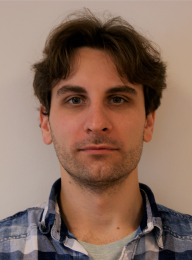
\includegraphics[width=\linewidth]{photo.png}
	\end{minipage}
	
	
	\section*{Objective}
	
	Data Science/Lead Data Science, Development
	
	\section*{Relevant skills}
	
	\setlength{\parindent}{3em}

	
I am Data Scientist with extensive experience in both Research and Development with focus on product quality.
I use my skills to solve the most challenging tasks that improve business in the area of data analysis.
My experience summary is:
\begin{itemize}
    \item 5+ years of Data Science
    \item 8+ years of applied Development
    \item 2+ years of people management
    \item 5 years of academic research in Theoretical Physics (Quantum Physics) 
\end{itemize}

In different organizations I improved my skills in Digital Signal Processing, Machine Learning, Deep Learning and, also, Development. I have produced many product components and algorithmic solutions for business value, that were successfully deployed.
Under my direction as Data Science Team Leader data processing service was developed for analysis of geological data using deep learning models, where I have designed full infrastructure from processing raw data pipelines to DL/ML processing and model library.
Also, I have developed FastAPI service on parallel project. 


I have advanced development skills with Python including linting, CI/CD, FastAPI, Flask and others (see examples on \href{https://github.com/ArseniyShchepetnov}{GitHub}), ability to create interactive dashboards and asynchronous applications.
Other languages that are covered with my experience are C++, Fortran, R.

Academic research in physics provided a fundamental pillar and a useful tool for my development in Data Science.

For personal NLP project I have developed web scraping tool (ScraPy + MongoDB). I use it to improve my machine learning and deep learning skills.



\newpage


	\setlength{\parindent}{0em}
	\vspace{\verticalSpace}
	\section*{Employment history}

	% InovIntell
	\begin{minipage}[t]{\lmpratio\textwidth}
		February 2023 --- \\Now
	\end{minipage}
	\hspace{\horizontalSpace}
	\begin{minipage}[t]{\rmpratio\textwidth}
		\sectionMain{Data Scientist}\\
		\href{https://www.inovintell.com/}{<<InovIntell>>} (Data Science), Tbilisi, Georgia\\[0.1cm]	

Machine Learning and Data Science in application to pharmacy.

        \begin{itemize}
                \item 
Carried out NLP research project related to the analysis of committee discussions on drugs ranking. Results attracted interest from potential clients.
			\item 
(In progress) Perform research related to the application of variational autoencoders in the task of medical trial generation and heterogeneous data.
		\end{itemize}
    
	\end{minipage}	
	\vspace{\vSpace}


	% 3Commas
	\begin{minipage}[t]{\lmpratio\textwidth}
		November 2022 --- \\January 2023
	\end{minipage}
	\hspace{\horizontalSpace}
	\begin{minipage}[t]{\rmpratio\textwidth}
		\sectionMain{Data Scientist}\\
		\href{https://3commas.io/}{<<3Commas>>} (Data Science), Tbilisi, Georgia\\[0.1cm]		

Developed solutions for ML cryptocurrency trading and inner projects related to Data Science.

		\begin{itemize}
                \item 
During the first week in company, I developed a message classification model for customer support data analysis.

			\item 
I developed and deployed several model backtesting components.
		\end{itemize}
		
	\end{minipage}	
	\vspace{\vSpace}

 
	% PWC
	\begin{minipage}[t]{\lmpratio\textwidth}
		May 2021 --- \\October 2022
	\end{minipage}
	\hspace{\horizontalSpace}
	\begin{minipage}[t]{\rmpratio\textwidth}
		\sectionMain{Lead Data Scientist/Team Lead/Senior Consultant -> Manager}\\
		\href{https://www.pwc.ru/}{<<PWC>>} (Technology, Artificial Intelligence), Saint-Petersburg\\[0.1cm]		

I was leading and developing multiple Data Science projects related to Bayesian Networks, Deep Learning and Machine Learning.
Data Science format includes both algorithmic and software development.

		\begin{itemize}
                \item 
Developed MLOps architecture and code for Deep Learning models for well logs data analysis.
			\item 
Designed and developed software for Bayesian Networks using FastAPI plus serious optimizations of python library for Bayesian Networks.
			\item 
Well Logs retrieval research with Deep Learning models was done under my direction, the client was satisfied and results were used in geology.
                \item 
I hired 2 junior and 1 intern Data Scientists and in less than a year got 2 junior and 1 middle.
                \item 
Due to good performance I was promoted up to the Manager Grade.
                \item 
I held a speech on careers days in two universities.
		\end{itemize}
		
After rebranding in July the unit is called <<Digital Formula of Trust>>.
		
	\end{minipage}	
	\vspace{\vSpace}
	
	% IBM
	\begin{minipage}[t]{\lmpratio\textwidth}
		May 2018 --- \\May 2021
	\end{minipage}
	\hspace{\horizontalSpace}
	\begin{minipage}[t]{\rmpratio\textwidth}
		\sectionMain{Data Scientist/Lead Data Scientist/Team Lead}\\
		\href{https://www.ibm.com/ru/rstl/index-en.html}{<<IBM STC>>} (GBS, ``Cognitive Practice Team''), Saint-Petersburg, Moscow\\[0.1cm]
  
Consulting services in the area of Data Science and Artificial Intellegence.
Research and development of Data Science and AI solutions for clients.
  
		\begin{itemize}
                \item 
Developed models for searching oil intervals with Deep Learning and Machine Learning models.
Real oil was extracted in locations that models predicted.
                \item 
I carried out research on correlation of wells for spatial analysis and designed several models.
Predictions were used by the client.
                \item
Using bokeh package I have developed interactive dashboards for geological data, including GIS signals and layers visualizations and maps.
                \item
I developed model serving solutions for research optimization.
                \item
I grew from middle to senior Data Scientist and started leading a team.
            \end{itemize}
		
	\end{minipage}	
	\vspace{\vSpace}
	
	% Healbe
	\begin{minipage}[t]{\lmpratio\textwidth}
		Aug 2016 --- \\May 2018
	\end{minipage}
	\hspace{\horizontalSpace}
	\begin{minipage}[t]{\rmpratio\textwidth}
		\sectionMain{Research and Development}\\
		\href{https://healbe.com/}{<<Healbe corp.>>}, Saint-Petersburg\\[0.1cm]	
  
Research and Development of algorithms for the wearable device sensors.
		\begin{itemize}
                \item 
I developed algorithms for custom piezoelectric and optical devices which were successfully deployed.
                \item 
I developed several utilities for data transfer from wearable devices and applying algorithms on the local machine which were used also in parallel projects.
            \end{itemize}
		 
		
	\end{minipage}	
	\vspace{\vSpace}


        \begin{minipage}[t]{\lmpratio\textwidth}
		Nov 2013 --- \\Feb 2016
	\end{minipage}
	\hspace{\horizontalSpace}
	\begin{minipage}[t]{\rmpratio\textwidth}
		\sectionMain{Engineer-programmer}\\
		\href{http://www.rimr.ru/eng/}{<<Russian Institute for Power Radiobuilding>>}, Saint-Petersburg\\[0.1cm]
            \begin{itemize}
                \item
I developed PostgreSQL database and UI on C++/Qt4 which was successfully deployed for business on Linux.
            \end{itemize}

	\end{minipage}

		\vspace{\vSpace}
	
	% SPBSU	
	\begin{minipage}[t]{\lmpratio\textwidth}
		Jan 2015 --- \\Dec 2015
	\end{minipage}
	\hspace{\horizontalSpace}
	\begin{minipage}[t]{\rmpratio\textwidth}
		\sectionMain{Researcher}\\
		\href{http://english.spbu.ru/}{<<Saint-Petersburg State University>>}, Saint-Petersburg\\[0.5cm]		
		Research in the field of atomic physics, $g$ factor theory, nuclear recoil effect. \\

	\end{minipage}
	\vspace{\vSpace}

	\begin{minipage}[t]{\lmpratio\textwidth}
		Jan 2014 --- \\Dec 2016
	\end{minipage}
	\hspace{\horizontalSpace}
	\begin{minipage}[t]{\rmpratio\textwidth}
		\sectionMain{Researcher}\\
		\href{http://frrc.itep.ru/index.php/en/}{<<Institute for Theoretical and Experimental Physics>>}, Moscow\\[0.5cm]
		Research in the field of atomic physics supported by ``Helmholtz-Rosatom'' grant. 
		Theme: ``Zeeman splitting in highly-charged ions: novel approach to the non-linear effects''. \\[0.5cm]

        Using DKB-splines, Runge–Kutta and other numerical methods mainly in Fortran.
  
	\end{minipage}
	
	\vspace{\vSpace}

	
	
	\begin{minipage}[t]{\lmpratio\textwidth}
		Sep 2011 --- \\Jan 2012
	\end{minipage}
	\hspace{\horizontalSpace}
	\begin{minipage}[t]{\rmpratio\textwidth}
		\sectionMain{Teacher (Physics)}\\
		\href{http://lnmo.ru/}{<<Laboratory for Continuous Mathematical Education>>}, Saint-Petersburg\\[0.5cm]
		Teaching physics at 8 and 9 year classes. Special seminars on thermodynamics.
	\end{minipage}	
	\vspace{\verticalSpace}
%-------------------------------------------------------------------------------------------------------------------------------
	\vspace{\verticalSpace}
	\section*{Education}
	
	\begin{minipage}[t]{\lmpratio\textwidth}
		Sep 2013 --- \\Jul 2016
	\end{minipage}
	\hspace{\horizontalSpace}
	\begin{minipage}[t]{\rmpratio\textwidth}
		\sectionMain{Postgraduate student} (Theoretical Physics)\\[0.1cm]		
		\href{http://english.spbu.ru/}{Saint-Petersburg State University}\\ Department of Physics, Division of Quantum Mechanics
		 % Thesis: ``Nuclear recoil corrections to the $g$ factor of highly-charged ions'' \\[0.3cm]
		 % Scientific advisors: \href{http://fock.phys.spbu.ru/english/tupicin_en.htm}{Prof. Ilya Tupitsyn} and \href{http://fock.phys.spbu.ru/glazov.htm}{Dr. Dmitry Glazov}
	\end{minipage}

	\vspace{1cm}
	
	\begin{minipage}[t]{\lmpratio\textwidth}
		Sep 2011 --- \\Jul 2013
	\end{minipage}
	\hspace{\horizontalSpace}
	\begin{minipage}[t]{\rmpratio\textwidth}
		\sectionMain{Master's degree} (Quantum Mechanics of Atoms, Molecules and Solids) \\[0.1cm]
		\href{http://english.spbu.ru/}{Saint-Petersburg State University}\\ Department of Physics, Division of Quantum Mechanics
		 % Thesis: ``Nuclear recoil corrections to the energy levels and to the $g$ factor of highly-charged ions''\\[0.3cm]
		 % Scientific advisor: \href{http://fock.phys.spbu.ru/english/tupicin_en.htm}{Prof. Ilya Tupitsyn} and \href{http://fock.phys.spbu.ru/glazov.htm}{Dr. Dmitry Glazov}
	\end{minipage}

	\vspace{1cm}
	
	\begin{minipage}[t]{\lmpratio\textwidth}
		Sep 2007 --- \\Jul 2011
	\end{minipage}
	\hspace{\horizontalSpace}
	\begin{minipage}[t]{\rmpratio\textwidth}
		\sectionMain{Bachelor's degree} (Quantum Mechanics of Atoms, Molecules and Solids) \\[0.1cm]
		\href{http://english.spbu.ru/}{Saint-Petersburg State University}\\ Department of Physics, Division of Quantum Mechanics
		 % Thesis: ``Nuclear recoil corrections to the energy levels of highly-charged ions''\\[0.3cm]
		 % Scientific advisor: \href{http://fock.phys.spbu.ru/english/shabaev_en.htm}{Prof. Vladimir Shabaev}
	\end{minipage}
	
	\newpage
	
%-------------------------------------------------------------------------------------------------------------------------------
	\section*{Certificates}	

        \begin{minipage}[t]{\lmpratio\textwidth}
		Coursera\\August 2022
	\end{minipage}
	\hspace{\horizontalSpace}
	\begin{minipage}[t]{\rmpratio\textwidth}
		\sectionMain{Natural Language Processing Specialization}\\
            \href{https://www.coursera.org/account/accomplishments/specialization/certificate/D4F2WRLEHCY8}{D4F2WRLEHCY8}
	\end{minipage}
	\vspace{1cm}

        \begin{minipage}[t]{\lmpratio\textwidth}
		Coursera\\August 2022
	\end{minipage}
	\hspace{\horizontalSpace}
	\begin{minipage}[t]{\rmpratio\textwidth}
		\sectionMain{Natural Language Processing with Attention Models}\\
		\href{https://www.coursera.org/account/accomplishments/certificate/TT5J2NHDYDY2}{TT5J2NHDYDY2}
	\end{minipage}
	\vspace{1cm}

	\begin{minipage}[t]{\lmpratio\textwidth}
		Coursera\\August 2022
	\end{minipage}
	\hspace{\horizontalSpace}
	\begin{minipage}[t]{\rmpratio\textwidth}
		\sectionMain{Natural Language Processing with Classification and Vector Spaces}\\
		\href{https://www.coursera.org/account/accomplishments/certificate/3LL65SQH6EWM}{3LL65SQH6EWM}
	\end{minipage}
	\vspace{1cm}

	\begin{minipage}[t]{\lmpratio\textwidth}
		Coursera\\August 2022
	\end{minipage}
	\hspace{\horizontalSpace}
	\begin{minipage}[t]{\rmpratio\textwidth}
		\sectionMain{Natural Language Processing with Probabilistic Models}\\
		\href{https://www.coursera.org/account/accomplishments/certificate/C3RSRG7T853E}{C3RSRG7T853E}
	\end{minipage}
	\vspace{1cm}
	

	\begin{minipage}[t]{\lmpratio\textwidth}
		Coursera\\August 2022
	\end{minipage}
	\hspace{\horizontalSpace}
	\begin{minipage}[t]{\rmpratio\textwidth}
		\sectionMain{Natural Language Processing with Sequence Models}\\
		\href{https://www.coursera.org/account/accomplishments/certificate/667D47FVSK3M}{667D47FVSK3M}
	\end{minipage}
	\vspace{1cm}


	\begin{minipage}[t]{\lmpratio\textwidth}
		Coursera\\July 2022
	\end{minipage}
	\hspace{\horizontalSpace}
	\begin{minipage}[t]{\rmpratio\textwidth}
		\sectionMain{Combinatorics and Probability}\\
		\href{https://www.coursera.org/account/accomplishments/certificate/EFYQQQ9GUTUP}{EFYQQQ9GUTUP}
	\end{minipage}
	\vspace{1cm}

	\begin{minipage}[t]{\lmpratio\textwidth}
		Coursera\\June 2022
	\end{minipage}
	\hspace{\horizontalSpace}
	\begin{minipage}[t]{\rmpratio\textwidth}
		\sectionMain{Sample-based Learning Methods}\\
		\href{https://www.coursera.org/account/accomplishments/certificate/KC4T942AATVE}{KC4T942AATVE}
	\end{minipage}
	\vspace{1cm}

		
	\begin{minipage}[t]{\lmpratio\textwidth}
		Coursera\\May 2022
	\end{minipage}
	\hspace{\horizontalSpace}
	\begin{minipage}[t]{\rmpratio\textwidth}
		\sectionMain{Fundamentals of Reinforcement Learning}\\
		\href{https://www.coursera.org/account/accomplishments/certificate/U3NT5V7XZCNK}{U3NT5V7XZCNK}
	\end{minipage}
	\vspace{1cm}
		
	
%-------------------------------------------------------------------------------------------------------------------------------
	\section*{Publications}
	\begin{itemize}
		\item A.~A.~Shchepetnov, D.~A.~Glazov, A.~V.~Volotka, V.~M.~Shabaev, I.~I.~Tupitsyn, G.~Plunien 
			``Nuclear recoil correction to the $g$ factor of boron-like argon''. Journal of Physics: Conference Series, 2015. --- Vol. 583, --- P. 012001
		\item I.~A.~Aleksandrov, A.~A.~Shchepetnov, D.~A.~Glazov, V.~M.~Shabaev 
			``Finite nuclear size corrections to the recoil effect in hydrogenlike ions''. Journal of Physics B: Atomic, Molecular and Optical Physics, 2015. --- Vol. 48, --- No. 14. --- P. 144004		
		\item D.~A.~Glazov, A.~V.~Volotka, A.~A.~Schepetnov, M.~M.~Sokolov, V.~M.~Shabaev, I.~I.~Tupitsyn, G.~Plunien 
			``$g$ factor of boron-like ions: ground and excited states''. Physica Scripta, 2013. --- Vol. T156, --- P. 014014
	\end{itemize}
% 	New articles are in preparation. 
% 	\vspace{\verticalSpace}
% 	\newpage
	\section*{International conferences}
		\begin{itemize}
			\item[---]	Seminar on Astrophysics, Clocks and Fundamental Constants, Bad Honnef, Germany (Poster), 2015
			\item[---]	Topical Workshop of the SPARC Collaboration, Worms, Germany (Poster), 2014
			\item[---]	\href{http://indico.gsi.de/conferenceDisplay.py?confId=2443}{International Conference on Science and Technology for FAIR}, Worms, Germany (Poster), 2014
			\item[---]	\href{http://www.cab.cnea.gov.ar/hci2014/}{International Conference on the Physics of Highly Charged Ions}, San Carlos de Bariloche, Argentina (\textbf{Oral presentation}), 2014
			\item[---]	\href{https://sites.google.com/site/finqinternational/home}{Fin Q workshop}: International conference <<Quantum Informatics and Applications>>, St. Petersburg, Russia (No report), 2013
			\item[---]	\href{http://www.gao.spb.ru/russian/psas/ffk2013/}{The Workshop on Precision Physics and Fundamental Physical Constants}, Pulkovo, St. Petersburg, Russia (Poster), 2013
			\item[---]	\href{http://fas.vsu.ru/en/index.php}{XX Conference on Fundamental Atomic Spectroscopy}, Voronezh, Russia (\textbf{Oral presentation}), 2013
		\end{itemize}		
	
	\vspace{5cm}
	
	Arseniy Shchepetnov
	
	
	
	
\end{document}

